%%%%%%%%%%%%%%%%%%%%%%%%%%%%%%%%%%%%%%%%%%%%%%%%%%%%%%%%%%%
%
%    Basierend auf der Vorlage vom Prof. Braun, FHWS
%
%%%%%%%%%%%%%%%%%%%%%%%%%%%%%%%%%%%%%%%%%%%%%%%%%%%%%%%%%%%
\documentclass[12pt,oneside,a4paper,parskip]{scrbook}
\usepackage[utf8]{inputenc}
\usepackage[ngerman]{babel}
\usepackage[pdftex]{graphicx}
\usepackage[hidelinks]{hyperref}
\usepackage{color}
\usepackage{amssymb}
\usepackage{textcomp}
\usepackage{pdfpages}
\usepackage{float}
\usepackage{pdflscape}
\usepackage{pdfpages}
\usepackage[nouppercase,headsepline,plainfootsepline]{scrpage2}
\usepackage{listings}
\usepackage{xcolor}
\usepackage{caption}
\usepackage{epstopdf}
\usepackage{longtable}
\usepackage{setspace}
\usepackage{booktabs}
\usepackage[backend=bibtexu, style=numeric]{biblatex}

\usepackage{csquotes}
%\usepackage{floatflt}
%\usepackage{subfigure}
%\usepackage{nicefrac}
%\usepackage[verbose]{placeins} 



%%%%%%%%%%%%%%%%%%%%%%%%%%%%%%%
%    Literatur File           %
%%%%%%%%%%%%%%%%%%%%%%%%%%%%%%%
\bibliography{literatur2}


%%%%%%%%%%%%%%%%%%%
%% definitions
%%%%%%%%%%%%%%%%%%%
\def\BaAuthor{Oleg Geier\qquad Daniel Glück\qquad Jonas Kaiser \\Tobias Lediger\qquad Daniel Mügge}
\def\BaTitle{Entwicklung eines Spiels auf Basis von C++}
\def\BaSupervisorOne{Prof.\ Dr.\ Peter Braun}
\def\BaSupervisorTwo{Prof.\ Dr.\ Steffen Heinzl}
\def\BaDeadline{17.07.2015}

% Spielname
\newcommand{\gamename}{\textbf{Josie--A Jelly's Journey }}

\hypersetup{
pdfauthor={Oleg Geier, Daniel Glück, Jonas Kaiser, Tobias Lediger, Daniel Mügge},
pdftitle={\BaTitle},
pdfsubject={Programmierprojekt SS15},
pdfkeywords={Programming, C++, cocos2d}
}

%%%%%%%%%%%%%%%%%%%
%% configs to include
%%%%%%%%%%%%%%%%%%%
\colorlet{punct}{red!60!black}
\definecolor{background}{HTML}{EEEEEE}
\definecolor{delim}{RGB}{20,105,176}
\colorlet{numb}{magenta!60!black}

\definecolor{gray}{rgb}{0.4,0.4,0.4}
\definecolor{darkblue}{rgb}{0.0,0.0,0.6}
\definecolor{cyan}{rgb}{0.0,0.6,0.6}

\definecolor{pblue}{rgb}{0.13,0.13,1}
\definecolor{pgreen}{rgb}{0,0.5,0}
\definecolor{pred}{rgb}{0.9,0,0}
\definecolor{pgrey}{rgb}{0.46,0.45,0.48}


\usepackage{calc} 

\newlength\tdima 
\newlength\tdimb 
\newlength\offset
\setlength\offset{6pt}
\setlength\tdima{ \fboxsep+\fboxrule} 
\setlength\tdimb{-\fboxsep+\fboxrule+\offset} 


\definecolor{listinggray}{gray}{0.6}

\DeclareCaptionFont{white}{\color{white}}
\DeclareCaptionFormat{listing}{%
  \parbox{\textwidth}{\colorbox{listinggray}{\parbox{\textwidth-\offset}{#1#2#3}}\vskip+3pt}}
\captionsetup[lstlisting]{format=listing,labelfont=white,textfont=white}
\lstset{
frame = tlbr, %
columns=fullflexible, %
 xleftmargin = \tdima, %
 xrightmargin = \tdimb, %
 tabsize=4, %
 language=Java, %
 basicstyle=\scriptsize\ttfamily, %
 upquote=false, %
 numberfirstline=true, %
 numberblanklines=false, %
 numbers=left,%
 numberstyle=\tiny, % 
 stepnumber=1, %
 numbersep = 10pt, %
 float=tp, %
 breakautoindent = true,%
 %This tells latex to keep more distance to the element above
 %aboveskip={1.5\baselineskip}, 
 showstringspaces=false, %
 extendedchars=true,%
 prebreak = \raisebox{0ex}[0ex][0ex]{\ensuremath{\hookleftarrow}}, %
 showtabs=false, %
 showspaces=false,%
 linewidth=\textwidth,%
 showstringspaces=false, %
 identifierstyle=\ttfamily, %
 keywordstyle=\color[rgb]{0,0,1}, %
 commentstyle=\color{gray}\upshape
 stringstyle=\color{black}, %
 breaklines=true, %
 breakatwhitespace=true, %
 columns=fullflexible, % 
 xleftmargin=8.9mm,%                 % code einrücken (rückt nummern mit ein!)
 framexleftmargin=22pt,%                % box so schieben, dass nummern mit drin sind
 framexrightmargin = 0pt, %
 escapechar=\&,						% char to escape out of listings and back to LaTeX
 literate={«}{{\flqq{}}}1 {»}{{\frqq{}}}1 %
} 

\lstdefinelanguage{json}{
    basicstyle=\normalfont\ttfamily,
    numbers=left,
    numberstyle=\scriptsize,
    stepnumber=1,
    numbersep=8pt,
    showstringspaces=false,
    breaklines=true,
    backgroundcolor=\color{background},
    literate=
     *{0}{{{\color{numb}0}}}{1}
      {1}{{{\color{numb}1}}}{1}
      {2}{{{\color{numb}2}}}{1}
      {3}{{{\color{numb}3}}}{1}
      {4}{{{\color{numb}4}}}{1}
      {5}{{{\color{numb}5}}}{1}
      {6}{{{\color{numb}6}}}{1}
      {7}{{{\color{numb}7}}}{1}
      {8}{{{\color{numb}8}}}{1}
      {9}{{{\color{numb}9}}}{1}
      {:}{{{\color{punct}{:}}}}{1}
      {,}{{{\color{punct}{,}}}}{1}
      {\{}{{{\color{delim}{\{}}}}{1}
      {\}}{{{\color{delim}{\}}}}}{1}
      {[}{{{\color{delim}{[}}}}{1}
      {]}{{{\color{delim}{]}}}}{1},
}

\lstset{language=xml,
  morestring=[b]",
  morestring=[s]{>}{<},
  morecomment=[s]{<?}{?>},
  stringstyle=\color{black},
  numbers=left,
  numberstyle=\scriptsize,
  stepnumber=1,
  numbersep=8pt,
  identifierstyle=\color{darkblue},
  keywordstyle=\color{cyan},
  backgroundcolor=\color{background},
  morekeywords={xmlns,version,type}% list your attributes here
}

\lstset{language=Java,
  showspaces=false,
  showtabs=false,
  tabsize=4,
  breaklines=true,
  keepspaces=true,      
  numbers=left,
  numberstyle=\scriptsize,
  stepnumber=1,
  numbersep=8pt,
  showstringspaces=false,
  breakatwhitespace=true,
  commentstyle=\color{pgreen},
  keywordstyle=\color{pblue},
  stringstyle=\color{pred},
  basicstyle=\ttfamily,
  backgroundcolor=\color{background},
%  moredelim=[il][\textcolor{pgrey}]{$$},
%  moredelim=[is][\textcolor{pgrey}]{\%\%}{\%\%}
}

\lstdefinestyle{singleline}{
language=C++,
numbers=none,
frame=none,
backgroundcolor=\color{white},
belowcaptionskip=1\baselineskip,
basicstyle=\footnotesize\ttfamily,
aboveskip = 1em,
belowskip = 0em
}

%%%%%%%%%%%%%%%%%%%
%% Klassendiagramme, etc.
%%%%%%%%%%%%%%%%%%%
\usepackage{tikz}
\usetikzlibrary{positioning,shapes,shadows,arrows}

\pgfdeclarelayer{background}
\pgfdeclarelayer{foreground}
\pgfsetlayers{background,main,foreground}

% Draw background
\newcommand{\mybackground}[5]{
  \begin{pgfonlayer}{background}
    \path (#1.west |- #2.north)+(-0.5,0.5) node (a1) {};
    \path (#3.east |- #4.south)+(+0.5,-0.25) node (a2) {};	
    \path[fill=yellow!20,rounded corners, draw=black!50, dashed] (a1) rectangle (a2);
    \path (a1.east |- a1.south)+(1.5,-0.3) node (u1)[above, text width=8em] {#5};
  \end{pgfonlayer}}

\newcommand{\shortnode}[2]{
\node (#1) [#2]{
	\textbf{#1}};}

\tikzstyle{classobject}=[rectangle, draw=black, rounded corners, fill=blue!40, drop shadow,
        text centered, anchor=north, text=black, text width=9em]
\tikzstyle{scene}=[classobject, fill=red!40]
\tikzstyle{layer}=[classobject, fill=yellow]
\tikzstyle{static}=[classobject, fill=gray, text=white]
\tikzstyle{cocosclass}=[classobject, fill=lightgray]
\tikzstyle{line}=[thick,->,>=triangle 45]
\tikzstyle{subclassLine}=[thick,->,>=open triangle 90]

%%%%%%%%%%%%%%%%%%%
%% unsere LaTeX shortcuts
%%%%%%%%%%%%%%%%%%%

\newcommand{\josieclass}[1]{\mbox{\textit{#1}}}
\newcommand{\cocosclass}[1]{\mbox{\textit{cocos2d::#1}}}


\newcommand{\notebox}[1]{
\colorbox{black!10}{\begin{minipage}{\textwidth -18pt}
#1
\end{minipage}}}

\begin{document}


%%%%%%%%%%%%%%%%%%%
%% Titelseite
%%%%%%%%%%%%%%%%%%%


\frontmatter
\titlehead{%  {\centering Seitenkopf}
  {Hochschule für angewandte Wissenschaften Würzburg-Schweinfurt\\
   Fakultät Informatik und Wirtschaftsinformatik}}
\subject{Projektdokumentation}
\title{\BaTitle\\[15mm]}
\subtitle{\normalsize{vorgelegt an der Hochschule f\"{u}r angewandte Wissenschaften W\"{u}rzburg-Schweinfurt in der Fakult\"{a}t Informatik und Wirtschaftsinformatik zum Abschluss des Programmierprojekts im vierten Studiensemester im Studiengang Informatik}}
\author{\BaAuthor}
\date{\normalsize{Eingereicht am: \BaDeadline}}
\publishers{
  \normalsize{Erstpr\"{u}fer: \BaSupervisorOne}\\
  \normalsize{Zweitpr\"{u}fer: \BaSupervisorTwo}\\
}

%\uppertitleback{ }
%\lowertitleback{ }

\maketitle


%%%%%%%%%%%%%%%%%%%
%% abstract
%%%%%%%%%%%%%%%%%%%

\section*{Zusammenfassung}

TODO

%%%%%%%%%%%%%%%%%%%
%% Inhaltsverzeichnis
%%%%%%%%%%%%%%%%%%%
\tableofcontents										



%%%%%%%%%%%%%%%%%%%
%% Main part of the thesis
%%%%%%%%%%%%%%%%%%%
\mainmatter

\chapter{Einleitung}\label{ch:intro}

\sectionDM{Ausgangssituation}\label{sec:1_Ausgangssituation}

In der heutigen Zeit spielt man Videospiele nicht nur auf Computern oder Konsolen, sondern auch auf Mobiltelefonen. Der Markt von Spielen für mobile Geräte ist in den letzten Jahren rapide gewachsen und erfreut sich immer größerer Beliebtheit. Einer Studie von Bitkom \cite{bitkomgaming} aus dem Jahr 2014 zufolge, in der die beliebtesten Spieleplattformen ermittelt wurden, führt das Smartphone bzw. Handy mit 78\% um 9\% gegenüber dem stationären PC und ist somit an erster Stelle. Dieselbe Studie hat sich auch mit den beliebtesten und meist gespielten Spielegenres beschäftigt. Stratiegie- und Denkspiele sind laut Bitcom am beliebtesten, gefolgt von Gelegenheitsspielen, Actionspielen, Social Games, Jump n' Runs und Renn- und Sportspielen.




\sectionDM{Motivation}\label{sec:1_Motivation}

Im bisherigen Verlauf unseres Informatik-Studiums hatten wir wenig mit GUI oder Grafik im allgemeinen Sinne zu tun. Die meiste Zeit sehen wir Konsolenausgaben in weiß auf schwarz, ein wenig Textausgabe und das war es dann auch schon. 

Wir wollten etwas entwickeln mit dem wir im späteren Leben höchstwahrscheinlich nur noch als Anwender zu tun haben. Ein Spiel. 

Viele Informatik Studenten träumen oder haben davon geträumt ein Spieleentwickler zu werden. Doch meistens wird daraus nichts. Deshalb haben wir uns gedacht bevor wir ins wirkliche Berufsleben einsteigen, wollen wir einmal ein eigenes Spiel entwickeln und haben es \gamename getauft.


\newpage
\sectionDM{Vorgehen}\label{sec:1_Vorgehen}

Am Anfang war das Nichts.

Eine der schwierigsten Phasen in unserem Projektverlauf war das grobe Design. Wir wollten dass  \gamename jedem aus unserer Gruppe gefällt und jeder seine Ideen einbringen kann. Deshalb wurden die ersten zwei Wochen des Projekts dem Design gewidmet. 

Nachdem wir wussten welche Komponenten für die Enwicklung benötigt werden, haben wir die Aufgabenbereiche auf die Team-Mitglieder wie folgt verteilt.

\begin{itemize}

\item Oleg Geier: Programmierung und Logik

\item Daniel Glück: Grafikdesign und Spieldesign

\item Jonas Kaiser: Spieldesign und Levelgenerierung

\item Tobias Lediger: Storydesign und Zwischensequenzen

\item Daniel Mügge: Audiodesign und Grafikdesign
	
\end{itemize}



\sectionDM{Dokumentationsstruktur}\label{sec:1_Dokumentationsstruktur}
Im \href{ch:grundl}{nächsten Kapitel} werden die Grundlagen erklärt. Diese beinhalten eine Anleitung zur Einrichtung der Entwicklungsumgebung und Einbindung der verwendeten Engine, eine grobe Einführung in die wichtigsten Bestandteile dieser und wie diese in unserem Programm eingesetzt wurden. 
Kapitel \ref{ch:arch} zeigt die Struktur des Spiels und das Zusammenspiel der Klassen und deren Abhängigkeiten mit Hilfe von Diagrammen.
In Kapitel \ref{ch:impl} geben kleine Code--Beispiele einen Einblick über die Implementierung der zur Verfügung stehenden Klassen und Methoden in den Programmcode.
Kapitel \ref{ch:eval} beschäftigt sich mit der Evaluation des Projektes im Hinblick auf das was geschafft und wie gut es umzusetzten wurde, auf den Ablauf des Projektes und die Probleme die während der Entwicklung enstanden, gelöst oder nicht gelöst wurden.
Kapitel \ref{ch:fazit} enthält Ausblicke für die Zukunft des Projektes und ein abschließendes Fazit.



\chapter{Grundlagen}\label{ch:grundl}



\sectionDM{Spielprinzip von Josie - A Jelly's Journey}
\gamename  erinnert an eine erweiterte Version des Spieleklassikers Super Mario World.
In der Theorie sollte es mehrere Spielabschnitte geben, jedoch wurde aus zeitlichen Gründen nur ein Abschnitt implementiert. Ein Spielabschnitt besteht aus drei Jump and Run Levels und einem Boss Kampf Level. 

\paragraph{Jump and Run Level:}
Der Spieler versucht ohne Zeiteinschränkung das Level abzuschließen und dabei so viele Münzen wie möglich zu sammeln. Bei einem perfekten Lauf \textbf{kann} man alle Münzen einsammeln, einige davon sind allerding so plaziert dass sie nur schwer zu erreichen sind.
Dem Spieler stehen die Steuerungsfunktionen "'Stoppen"', "'Schrumpfen"' und "'Springen"' zur Verfügung. 
Dass Josie von selbst in einer festgelegten Geschwindigkeit läuft, führt zu einer gewissen Schwierigkeit des Spiels und macht Steuerungsfunktionen für "'Links"' und "'Rechts"' überflüssig.

\paragraph{Boss Level:}



\sectionTL{Framework}\label{sec:2_Framework}
Als die grobe Idee für das Spiel feststand, mussten wir uns für eine GameEngine entscheiden. Zur Auswahl standen unter anderem die AndEngine, Unity und Cocos2d-x. Nach ausreichender Recherche über die Funktionalitäten der verschiedenen Engines haben wir uns einstimmig für Cocos2d-x entschieden. Cocos2d-x untestützt drei Programmiersprachen, C++, JavaSkript und Lua. Hier haben wir C++ gewählt, da wir im laufe unseres Studiums eine Vorlesung über C++ gehört haben.
Die nächste Herausforderung war die Einrichtung von Cocos2d-x. Da wir drei verschiedene Betriebssysteme(Win8, MacOSX, Ubuntu) benutzen, hatten wir geringe Kompatibilitätsprobleme.
Um Cocos2d-x einzurichten, werden folgende Pakete benötigt:

\begin{itemize}
\item Cocos2d-x Link - \url{http://www.cocos2d-x.org/download}
\item Android SDK - \url{http://developer.android.com/sdk/index.html}
\item Android NDK - \url{http://androids.zone/android-ndk/#.VBLHNPldWXY}
\item Apache Ant - \url{http://ant.apache.org/bindownload.cgi}
\item Python - \url{https://www.python.org/downloads/}
\item Eclipse – \url{https://eclipse.org/downloads/}
\end{itemize}

Nachdem die Pakete heruntergeladen und ausgepackt sind, verschiebt man diese in den selben Ordner. Apache Ant und Python müssen installiert werden. Bei Python muss darauf geachtet werden das es sich um Version 2.x handelt. Unter Ubuntu muss Python nicht installiert werden, da dies schon in den Paketquellen vorhanden ist. 
Hat man die zwei Programme installiert öffnet man den Cocos2d-x Ordner und startet die setup.py Datei (über das Terminal). Daraufhin öffnet sich ein Terminalfenster in dem die Umgebungsvariablen angepasst werden, dies bedeutet man wird nach den Pfaden von der Android SDK/NDK, Apache Ant und Python gefragt. Entweder man gibt diese per Hand ein oder zieht die jeweiligen Ordner in das Terminalfenster. 



\sectionTL{IDE und Plugins}\label{sec:2_IDE}

Nachdem die Umgebungsvariablen eingetragen sind, muss das Android Developer Tool Plugin für Eclipse installiert werden. Hat man das erledigt öffnet man den im Plugin enthaltenen Android SDK-Manager und lädt sich hier nochmal die passende API herunter. In unserem Fall war das die API für Androidversion 4.4.2(API 19). 
Ist dieser Schritt geschafft, wird es Zeit das erste Projekt zu erstellen.
Hierzu öffnet man einen Terminal und wechselt in das Verzeichnis in dem auch der Cocos2d-x Ordner liegt. Hier gibt man folgenden Befehl ein:
	
\begin{lstlisting}[style=singleline]
	$cocos new MyGame -p com.MyCompany.MyGame -l cpp -d ~/MyCompany
\end{lstlisting}
		
\begin{itemize}
\item MyGame gibt den Namen des Projekts an
\item com.MyCompany.MyGame ist der Paketname für Android
\item cpp steht für die Programmiersprache. cpp für C++ und lua für Lua
\item ~/MyCompany gibt das Verzeichnis an in dem das Projekt gespeichert wird 
\end{itemize}

Der somit erstelle Ordner wird ins Git-Repository hochgeladen. 
Nun öffnet man wieder Eclipse und importiert das Git-Repository sowie die Cocos2d-x Bibliotheken. 

	Git-Repository: Eclipse → File → Import... → Git → 'Projects from Git'

Hier wählt man das vorher erstellte Projekt im Git-Repository aus.

	Cocos2d-x Bibliotheken: Eclipse → Import... → Android → 'Existing Android Code into 	Workspace'

Hier dirigiert man in das Verzeichnis in dem der Cocos2d-x Ordner liegt und wählt diesen komplett aus. Im nachfolgenden Fenster wählt man alle vorgeschlagenen Punkte ab bis auf libcocos2dx Nachdem beide 'Projekte' importiert wurden, wählt man sein Projekt aus dem Git-Repository aus und wechselt in die Einstellungen. Unter dem Reiter 'Android' ist darauf zu achten, dass als Library das Projekt libcocos2dx ausgewählt ist. Ist es nicht in der Liste enthalten, fügt man es mit 'Add' hinzu. 

Es ist darauf zu achten, dass sich alle Ordner inkl. dem Git-Repository in einem Ordner befinden.

Zu guter Letzt, öffnet man die AndroidManifest.xml in Eclipse aus und ändert hier den Wert auf die Entsprechende API.
\begin{lstlisting}[style=singleline]
	<uses-sdk android:minSdkVersion="19"
			  android:targetSdkVersion="19"/>
\end{lstlisting}
	

Nun kann man anfangen zu arbeiten! 



\sectionTL{Szenenprinzip}\label{sec:2_Szenenprinzip}
Eine Szene ist im Grunde genommen nichts anderes als ein Container, welcher  Sprites, Labels, Nodes und andere Objekte beinhaltet die ein Spiel benötigt. Eine Szene ist für die laufende Spiellogik und Darstellung des Inhaltes auf einer 'per-frame basis' verantwortlich. Es wird mindestens eine Szene benötigt damit man das Spiel starten kann. Man kann beliebig viele Szenen-Objekte in einem Spiel verwenden und leicht zwischen diesen überleiten. Der Vorteil von Szenen liegt darin, dass man nicht jedes Objekt einzeln laden muss. An eine Szene lassen sich diverse Sprites, Labels und Nodes mit der von Cocos2d-x gegebenen Funktion addChild() anhängen(siehe Abbildung \ref{fig:szenengraph}). Sobald das Szenen-Objekt geladen wird, werden die angefügten Kinder mitgeladen. Dies spart Zeit und entlastet den Speicher.

\begin{figure}[H]
  \centering
  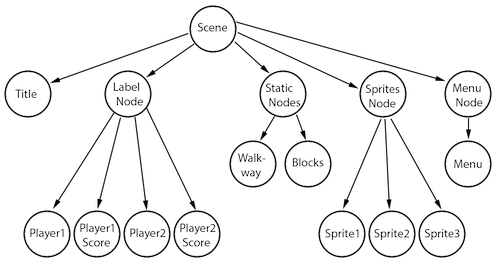
\includegraphics[width=12cm]{resources/scenegraph}
  \caption{Szenengraph}
  \label{fig:szenengraph} 
\end{figure}


\subsection{Szenenfunktionen von cocos2d}

Cocos bietet Funktionen an um Szenen zu erstellen und zwischen diesen zu wechseln. Um einen Szenenwechsel durchzufüren, muss zuerst eine Szene erstellt werden.

\begin{lstlisting}[style=singleline]
	Szene* Cutscene = Szene::create();
\end{lstlisting}


Dies erstellt ein Objekt des Typ Szene mit dem Namen Cutscene.
Im Laufe des Spiels ist es  notwendig zwischen den verschiedenen Szenen zu wechseln. Dies wird deutlich, wenn man z.B. ein neues Spiel starten oder ein anderes Level auswählen möchte. Hierzu stellt Cocos2d-x verschiedene Funktionen bereit eine Szene zu wechseln.

\begin{itemize}
\item replaceScene() ersetzt eine Szene vollständig durch eine Andere
\item pushScene() unterbricht die Ausführung der aktuellen Szene und verschiebt diese auf den Stack. Der Stack ist eine Art Warteschlange welche nach dem 'Last in, First out – Prinzip', dort wartet die Szene auf weitere Anweißungen. Diese Funktion darf nur aufgerufen werden, wenn bereits eine Szene aktiv ist.
\item popScene() wiederum ersetzt die aktuelle Szene und löscht diese komplett. Diese Funktion darf nur aufgerufen werden, wenn bereits eine Szene aktiv ist.
\end{itemize}



\sectionDG{Spriteprinzip}\label{sec:2_Spriteprinzip}
Allgemein betrachtet kann man sagen, dass ein Sprite(engl. Kobold, Geistwesen) ein Grafikobjekt ist, welches über den Hintergrund gelegt wird und von der Grafikhardware platziert wird. 
Der Name rührt daher, dass ein Sprite auf dem Bildschirm umherspäht und im Grafikspeicher nicht zu finden ist. Heutzutage bezeichnet der Begriff “Sprite” jedoch alle Objekte die so aussehen wie ein solches Grafikobjekt, jedoch eigentlich von einer Software erzeugt werden und im Grafikspeicher vorliegen. 
Solche softwareerzeugten Sprites sind streng genommen “Shapes”, für deren Erzeugung überwiegend die CPU zuständig ist.
 
Für Computerspiele sind mit Sprites einige Vereinfachungen verbunden. So werden zum Beispiel in vielen 2D Jump and Run Spielen so genannte Tiles oder auch Kachelgrafiken verwendet, welche ebenfalls kleine Grafikelemente sind die zusammengesetzt eine größere Grafik ergeben. Ihr Anwendungsbereich findet sich unter anderem im Aufbau eines Levels, wobei aus ihnen die Spielwelt zusammengesetzt wird.

\subsection{cocos2d Spriteprinzip}
In der von uns verwendeten Gameengine cocos2d, ist ein Sprite ein “Bild”, welches durch Veränderung seiner Werte manipuliert werden kann. Es gibt verschiedene Wege ein Sprite zu erstellen, je nach dem wozu es benutzt werden soll. Bezüglich Dateiformaten werden von cocos2d PNG, JPEG, TIFF etc. unterstützt. Wir haben uns für das Dateiformat PNG entschieden, da es eine gute Komprimierung, gute Qualität, Darstellung von Halbtransparenzen, also 50\% Deckraft, vorweist und außerdem ein sehr weit verbreiteter Datentyp ist.

Es gibt unterschiedliche Methoden ein Sprite zu erstellen. Eine Möglichkeit ist das Sprite aus einem Bild zu laden, wobei das in cocos2d erstellte Sprite Objekt die selben Abmessungen wie das benutzte Bild vorweist. 

\begin{lstlisting}[style=singleline]
Sprite* mySprite = Sprite::create("mysprite.png");
\end{lstlisting}

Eine weitere Methode ist das Erschaffen eines Sprites durch Angabe eines Ausschnittes des benutzten Bildes. Dabei wird im Erstellungsprozess ein so genanntes \texttt{Rect} angegeben, welches die Position als auch die Dimension auf dem Bildschirm darstellt. 

\begin{lstlisting}[style=singleline]
Sprite* mySprite = Sprite::create("mysprite.png", Rect(0,0,40,40));
\end{lstlisting}

Die Möglichkeit ein Sprite aus einem Spritesheet zu erstellen ist besonders empfehlenswert. Ein Spritesheet ist eine Bilddatei in der mehrere Sprites beliebig aneinander gereiht gespeichert werden können. Dies birgt den Vorteil, dass nur eine Datei geladen werden muss anstatt viele einzelne Bilder, was die Ladezeiten erheblich verringert und zudem eine Speicherreduktion mit sich bringt. Außerdem reduzieren diese die Aufrufe an OpenGL ES etwas zu zeichnen und zu rendern. Beim erstmaligen verwenden eines Spritesheets, wird dieses in den \cocosclass{SpriteFrameCache} geladen. Dies ist eine Klasse, welche ein \cocosclass{SpriteFrame} Objekt, für zukünftigen Schnellzugriff speichert. SpriteFrame-Objekte beinhalten den Bildnamen des Sprites und ein \texttt{Rect} um die Größe des Sprites zu spezifizieren. Aus dem SpriteFrameCache, in welchem das Spritesheet geladen wurde, kann nun ein Sprite erstellt werden.
Spritesheets stellen in unserem Projekt speziell für Animationen und die Umgebung der Spielwelt eine optimale Lösung dar. 



\subsection{Möglichkeiten Sprites zu manipuliern}
Der Ankerpunkt eines Sprites ist ein Punkt, welcher zur Orientierung bei der Positionsbestimmung eines Sprites dienen soll. Der Ankerpunkt benutzt ein Koordinaten System das von 0 bis 1 geht, wobei \texttt{0,0} unten links und \texttt{1,1} oben rechts vom Sprite ist.

\begin{lstlisting}[style=singleline]
Sprite* mySprite->setAnchorPoint(0,0); // (0,1), (1,0), (0.5,0.5)
\end{lstlisting}

\begin{figure}[H]
  \centering
  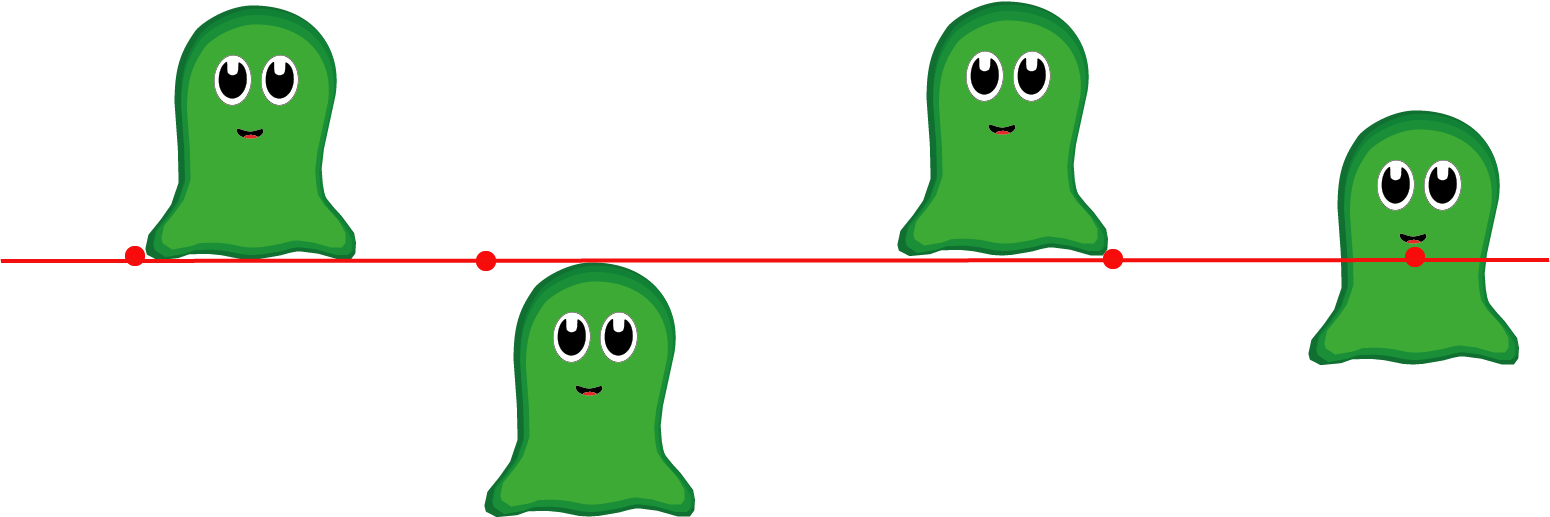
\includegraphics[width=10cm]{resources/josiedoku3}
  \caption{Plazierung von Josie bei verschiedenen Ankerpunkten (rot)}
  \label{fig:josie_ancherpoint} 
\end{figure}

Möglichkeiten ein Sprite zu manipulieren sind unter anderem Skalieren, Rotieren und Verzerren. Weiterhin kann man die Farbe und Sichtbarkeit eines Sprites verändern. Die in unserem Projekt am häufigsten verwendete Manipulationsmethode ist das Skalieren. Sie ermöglicht es die Größe eines Sprites beliebig zu verändern.

\begin{figure}[H]
 \centering
  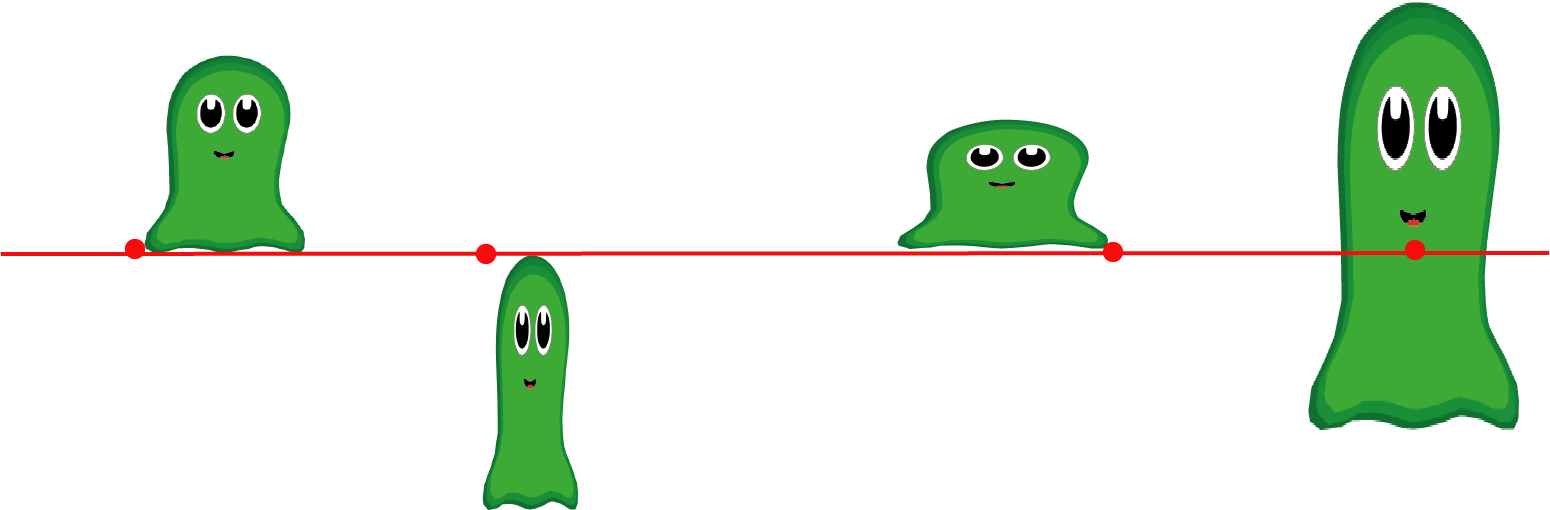
\includegraphics[width=10cm]{resources/josiedoku4}
  \caption{Josie nach dem Skalieren}
  \label{fig:josie_scale} 
\end{figure}



\sectionDG{Animationsprinzip}\label{sec:2_Animationsprinzip}

\subsection{Allgemeines und cocos2d Spriteprinzip}
Im Verlauf unseres Projektes wurden verschiedenste Animationen benutzt. Im folgenden soll ein kurzer Einblick in das Prinzip der Animationen in cocos2d, als auch allgemein gewährt werden. Einfach gesagt sind Animationen nichts weiter als eine sehr schnell abgespielte Aneinanderreihung von Bildern. In der Computergrafik oder bei Computerspielen werden diese verwendet um den Spielecharakter zum Leben zu erwecken und das Spiel dynamischer zu machen. Ohne sie wären Spiele nicht grafisch darstellbar.

In cocos2d werden solche Animationen durch \cocosclass{Action} Objekte realisiert. Diese haben die Fähigkeit die Werte von \cocosclass{Node} Objekte, in Echtzeit zu transformieren. Dazu zählen ebenfalls Instanzen der Klassen die von einem solchen Objekt erben. Werte eines Nodes, die verändert werden können sind z.b. die Sichtbarkeit, Farbe, Position oder auch die Größe des Nodes. Zum Beispiel kann ein Sprite von einer Position zur anderen bewegt werden.

Grundsätzlich können zwei Versionen von Actions unterschieden werden, diese sind By und To. Wobei Letztere absolut sind und im Gegensatz zu By Actions d.h. sie berücksichtigen die aktuelle Position des Node nicht. Ein mögliches Beispiel für eine MoveTo Animation soll im folgenden kurz beschrieben werden. Man erstellt ein MoveBy Objekt mit einer Angabe über die Dauer der Animation in Sekunden sowie ein Vektor der die Ziel Koordinaten auf der X als auch die der Y Achse beinhaltet. Anschließend wird dieses Objekt auf einem Node z.b. ein Sprite durch die Methode \textbf{runAction()} ausgeführt. 

\begin{figure}[H]
 \centering
  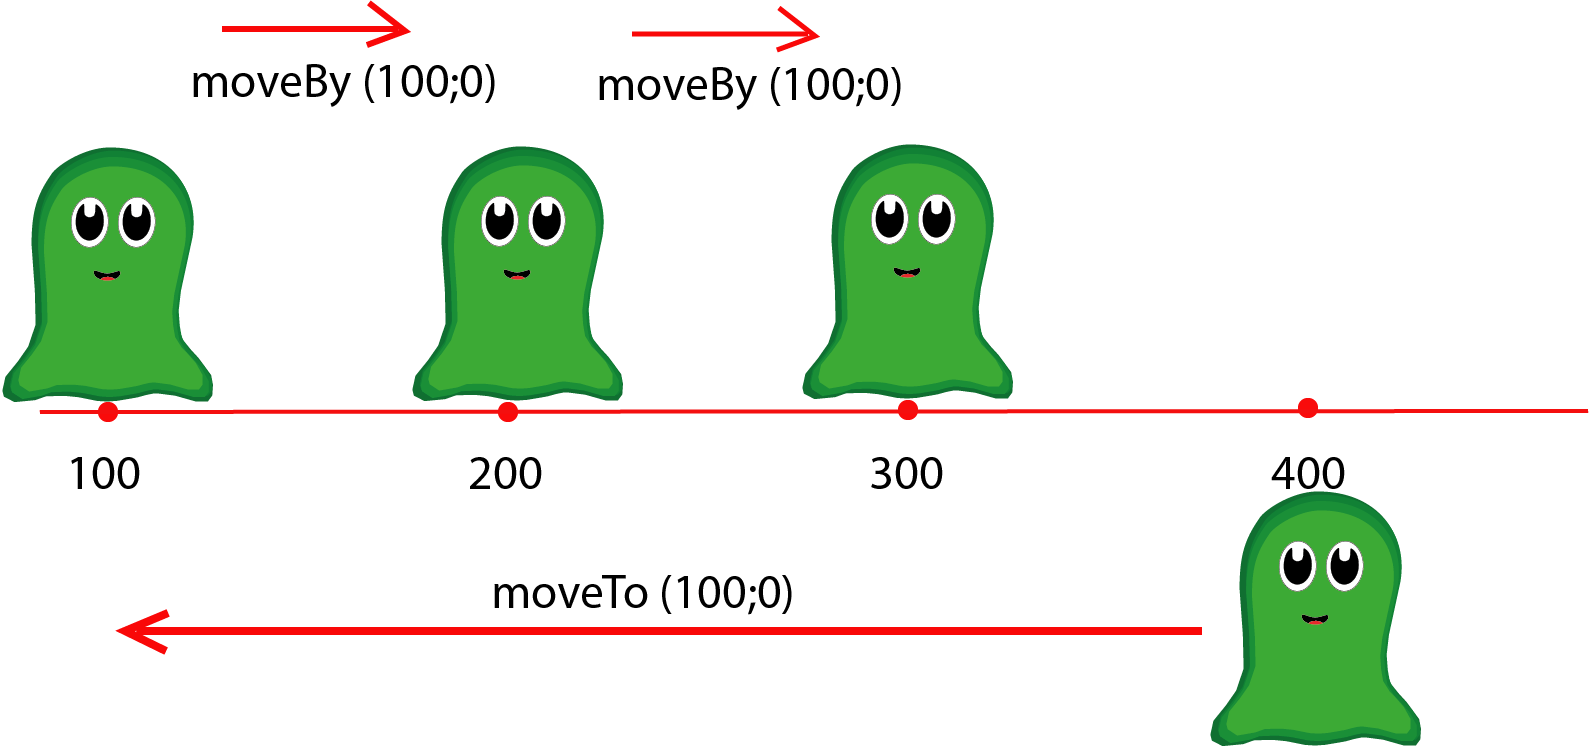
\includegraphics[width=10cm]{resources/josiedoku6}
  \caption{Unterschied zwischen MoveBy und MoveTo}
  \label{fig:josiemoveByTo} 
\end{figure}

Die von cocos2d bereitgestellten Funktionen zur Veränderung von Nodes sind Move, Rotate, Scale, Fade In/Out und Tint.

\begin{figure}[H]
 \centering
  
\includegraphics[width=10cm]{resources/josiedoku5}
  \caption{Beispiel für Fade In/Out bei Josie}
  \label{fig:fade} 
\end{figure}


\subsection{Animate und Sequenze}
Im vorangegangenen Abschnitt wurden ein Überblick einiger cocos2d bereitgestellter Animationen geschaffen. Im Verlauf eines Spieleprojektes wäre es jedoch sinnvoll eigene Animationen erstellen zu können. Eine Möglichkeit eigene Animationen zu erstellen wie zum Beispiel eine Art simples Daumenkino, bietet die Klasse \cocosclass{Animate}. Ein Animate enthält eine Animation bzw. wird aus dieser Erstellt. Animations sind Container welche durch die SpriteFrame Verzögerungszeit zwischen den Frames als auch die Dauer der Action bestimmt werden. Wenn ein Animate Objekt ausgeführt wird, werden bestimmte Frames auf dem Display durch die in dem Animate enthaltenen, ersetzt. So kann zum Beispiel ein SpriteFrame durch ein Set von SpriteFrames ersetzt werden.

Um Komplexe Abläufe von Animationen zu definieren ist es sinnvoll eine Klasse wie \cocosclass{Sequence} zu benutzen. Die Instanz einer Sequence ermöglicht es verschiedene Action, Function und sogar Sequence Objekte hintereinander zu reihen und in einem Sequence-Objekt zusammenzufassen. So können Abläufe von Animationen zusammengefasst werden.

\begin{figure}[H]
 \centering
  
\includegraphics[width=10cm]{resources/sequence}
  \caption{Beispiel für Sequenzen}
  \label{fig:sequence} 
\end{figure}

Ein Zusammenspiel von Grundfunktionen und Sequenzen fand in unserem Projekt bei den Angriffspattern des Boss Gegners Anwendung. Hierbei war ein Problem, dass sich bei zu kurzem Puffer und zu langen Aktionszeiten die einzelnen Aktionen vermischen.

Eine weitere Vereinfachung durch cocos2d bietet die Reverse Methode. Diese dient dazu Animationen rückwärts ablaufen zu lassen. Diese ist in unserem Projekt unter anderem bei der Sprung Animation zum Einsatz gekommen.


\subsection{Spritesheet}

Eine häufige Methode zur Spriteerstellung ist es das Spritesheet bei der Erzeugung in den Cache zu laden. 
Hierzu benötigt man nicht nur das Spritesheet sondern auch eine beschreibende “.plist” Datei, die eine Zuweisung von SpriteFrame zu Bildern und deren Position im Spritesheet enthält. Nun kann man einerseits durch ein Zusammenspiel zwischen Spritesheet und .plist Datei die Animation bzw. den Ablauf im eigenen Programm definieren. Hierbei werden die SpriteFrame und die .plist Datei geladen, um im Anschluss die SpriteFrames in der .plist Datei mit den Sprites aus dem Spritesheet zu koppeln. Andererseits kann man den Ablauf einer Animation in der .plist Datei festlegen und im Anschluss die fertige Animation laden.

Wir entschieden uns für die Spritesheet .plist Methode, da wir ebenfalls bei der Realisierung des Levels mit Spritesheets arbeiteten und die Arbeit mit diesen daher kennen. Bei der Suche nach einem Programm für die “Datei Methode” fanden wir weiterhin nur schlechte Tutorials.



\sectionOG{Datenkommunikation}

\subsection{Callbackprinzip}\label{sec:2_Callbackprinzip}
In vielen Teilen des Spieles wird \textbf{CC\textunderscore CALLBACK\textunderscore 0()} verwendet - unter anderem für Menü-Buttons. Ein Callback wird verwendet um einer Funktion, eine andere Funktion als Parameter zu übergeben. Im Besonderen wenn vorher nicht klar ist, wann diese Funktion ausgeführt wird (bsp. Klick auf einen Button). Genau genommen ist es nur ein Makro für die C\texttt{++} Funktion \textbf{std::bind}. Anstatt der Null könnte man auch eine Eins angeben um zusätzlich den Sender als Parameter zu übergeben.

Hier sei noch kurz das \textbf{CallFuncN} erwähnt. Das Callback wird in eine \cocosclass{Action} gekapselt, um die Funktion innerhalb einer Animations Sequenz auszuführen (S: \pageref{lst:CallFuncN}).


\subsection{Observer Pattern}

Für die Spielersteuerung (Kapitel \ref{sec:4_SpielerSteuerung}) wird ein Observer Pattern verwendet. Auch hier ist der Hintergrund die asynchrone Abarbeitung von Benutzer Ereignissen. Im Unterschied zum Callback geht es beim Observer immer um mindestens zwei Objekte, dem der die Nachricht sendet und dem der sie empfängt. Es können aber sowohl mehrere Empfänger (bsp. Radio), als auch mehrere Sender (bsp. Tempomat und Fahrer beeinflussen die Geschwindigkeit) beteiligt sein.

\begin{figure}[H]
 \centering
  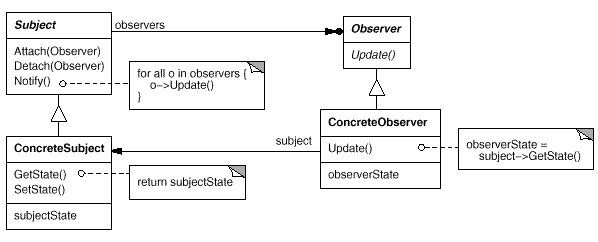
\includegraphics[width=15cm]{resources/observer_pattern}
  \caption{Aus dem Buch Design Patterns \cite[Seite 326ff]{gamma2011patterns}}
  \label{fig:observer_pattern} 
\end{figure}

Der Empfänger trägt sich selbst in eine Liste von Empfängern für ein bestimmtes Event/Namen ein und meldet somit sein Interesse für das Ereignis. Bei Eintreffen des Ereignisses geht der Sender die Liste der Empfänger durch und informiert jeden über das neue Ereignis.



\sectionJK{Tilemaps}\label{sec:2_Tilemaps}



\sectionDM{Musik und Sound-Effekte}\label{sec:2_Musik}
Musik sowie alle Sounds die in unserem Spiel \gamename zu hören sind wurden selbst geschrieben, aufgenommen und bearbeitet. Dazu gehören:

\begin{itemize}
\item Hintergrundmusik im Hauptmenü, in der Levelauswahl, in den Jump and Run Levels und im Boss Kampf
\item Effektsounds für Sprung--, Schrumpf--, Stop und Schuss--Sounds von Josie, Shop--Sound, Bosstreffer--Sound
\end{itemize}


\subsection{Möglichkeiten der cocos2d-x-Engine zur Audioverarbeitung}
Cocos2d bietet mit der \textbf{SimpleAudioEngine} eine relative einfache Möglichkeit Audio\-dateien, sei es die Hintergrundmusik oder ein Sound-Effekte, zu laden, abzuspielen, zu pausieren und wieder zu entfernen. Hierzu ein kurzes Beispiel wie man auf einfache Art und Weise eine Audiodatei abspielt.

\begin{lstlisting}[style=singleline]
SimpleAudioEngine::getInstance()->playBackgroundMusic("song.mp3",true);
\end{lstlisting}

Auf die Implementierung und die Verwendung der \cocosclass{SimpleAudioEngine} innerhalb unseres Codes wird im Kapitel \ref{sec:4_Audiounit} genauer eingegangen. Vorweg sei gesagt dass wir alle Funktionalitäten welche die \cocosclass{SimpleAudioEngine} betreffen in eine eigene Klasse \josieclass{AudioUnit} ausgelagert haben.


\subsection{Mono-/Stereo-Kanäle und Dateiformate}
Es ist möglich sowohl Mono-- als auch Stereo--Audiodateien zu verwenden. Falls man also möchte dass Sounds zum Beispiel aus bestimmten Richtungen kommen, um dem Spieler ein gewisses Mittendrin--Gefühl zu vermitteln, sollten die Audiodateien stereo sein. Das ist allerdings erst richtig sinnvoll wenn das Spiel mit Kopfhörern oder mit Anschluss an ein Soundsystem gespielt wird. 

In unserem Fall wurden Stereo--Audiodateien ohne Paning (mischen von Spuren nach links oder rechts) verwendet, da \gamename hauptsächlich für mobile Geräte gedacht ist und diese meist nur über einen Lautsprecher verfügen. In der Realität ist es außerdem meistens so, dass man bei Handyspielen den Ton ausschaltet bzw. ohne Kopfhörer spielt.

Wir haben auschließlich .mp3 verwendet, da dieses Dateiformat in Bezug auf cocos2d von den meisten Geräten unterstützt wird. Ein weiterer Vorteil von .mp3 gegenüber anderen Formaten wie .wav ist die Dateigröße, was im Bezug auf mobile Geräte ein sehr wichtiger Faktor ist.


\subsection{Audiobearbeitungsprogramme}
Auf dem Softwaremarkt gibt es unzählige Audiobearbeitungsprogramme. Wenn man sich mit dem Thema Audiobearbeitung noch nie beschäftigt hat, ist es sehr schwer eines zu finden das die nötigen Funktionen liefert um einen gutes Resultat zu erzielen. Zudem kosten die meisten guten Programme viel Geld. Im Folgenden soll eine Auflistung von einigen kostenplfichtigen und kostenlosen Programmen einen groben Überblick verschaffen:

\begin{itemize}
 \item Cubase (Steinberg, kostenpflichtig)
 \item Pro Tools (Avid, kostenpflichtig)
 \item Logic Pro (Apple, kostenpflichtig)
 \item Audacity (AudacityTeam, kostenlos)
 \item Goldwave (Goldwave Inc., teilweise kostenlos)
 \end{itemize} 

Bei \gamename wurde Logic Pro X von Apple verwendet. 

\chapter{Architektur}

\section{Klassenübersicht}\label{sec:Klassenuebersicht}

Beim Start des Spieles wird das AppDelegate aufgerufen, was wiederum augenblicklich die \textit{MainMenuScene} lädt. Dieser Bildschirm dient zum Einen (a) die \textit{Optionen} aufzurufen, (b) ein kurzes \textit{Tutorial} zur Erklärung der Steuerung und Hindernissen im Level, sowie (c) der eigentlichen Level Auswahl (\textit{LevelSelectScene}).
Die Level Auswahl unterscheided grundsätzlich zwischen einem normalen \textit{Level}, einem automatisch generierten (\textit{TMXEdit}) und dem Boss Kampf (mit vorgeschalteter \textit{ShopScene}).

\begin{figure}[h]
\scalebox{0.7}{\begin{tikzpicture}[node distance=0.8cm]

\shortnode{AppDelegate}{classobject}
\shortnode{MainMenuScene}{scene, right=of AppDelegate}
\shortnode{TutorialScene}{scene, right=of MainMenuScene}
\shortnode{OptionScreen}{layer, above=of TutorialScene}
\shortnode{LevelSelectScene}{scene, below=of MainMenuScene}
\shortnode{Cutscene}{scene, below=of LevelSelectScene}
\shortnode{TMXEdit}{classobject, left=1.5cm of Cutscene}
\shortnode{ShopScene}{scene, right=1.5cm of Cutscene}

\shortnode{LevelPlayer}{classobject, below=1.5cm of TMXEdit}
\shortnode{Level}{scene, right=of LevelPlayer}
\shortnode{LevelHUD}{layer, below=of Level}
\shortnode{StageHazard}{classobject, left=of LevelHUD}
\shortnode{MapController}{classobject, below=of StageHazard}
\shortnode{BossLevel}{scene, below=1.5cm of ShopScene}
\shortnode{BossPlayer}{classobject, right=of BossLevel}
\shortnode{BossLevelHUD}{layer, below=of BossLevel}
\shortnode{Projectile}{classobject, right=of BossLevelHUD}
\shortnode{PauseScreen}{layer, right=3.5cm of MapController}
\shortnode{LevelGameOver}{scene, below=1cm of MapController}

\shortnode{AudioUnit}{static, right=5cm of LevelGameOver}
\shortnode{GameStateManager}{static, right=1.5cm of AudioUnit, text width=4.2cm}

% draw lines
\draw[line] (AppDelegate.west) ++(-2,0) |- (AppDelegate.west);
\draw[line] (AppDelegate.east) |- (MainMenuScene.west);
\draw[line] (MainMenuScene.north) ++(0.8,0) |- (OptionScreen.west);
\draw[line] (MainMenuScene.east) |- (TutorialScene.west);
\draw[line] (MainMenuScene.south) -| (LevelSelectScene.north);
\draw[line] (LevelSelectScene.west) -| (TMXEdit.north);
\draw[line] (LevelSelectScene.south) -| (Cutscene.north);
\draw[line] (LevelSelectScene.east) -| (ShopScene.north);
\draw[line] (TMXEdit.south) -- ++(0,-0.5) -| ([xshift=-1cm]Level.north);
\draw[line] (Cutscene.south) -| (Level.north -| Cutscene.north);
\draw[line] ([xshift=1cm]ShopScene.south) -| ([xshift=1cm]BossLevel.north);
\draw[line, dotted] (TMXEdit.west) -- ++(-0.9,0) |- (MapController.west);
\draw[line, dashed] (LevelSelectScene.south -| Level.north) ++(-0.3,0) -| ([xshift=-0.3cm]Level.north);
\draw[line] (MapController.south -| MapController.east) ++(0.5,-0.2) -- ++(0,-0.3) -| (LevelGameOver.north);

\mybackground{LevelPlayer}{LevelPlayer}{LevelHUD}{PauseScreen}{Level Scene}
\mybackground{BossLevel}{BossLevel}{Projectile}{PauseScreen}{BossLevel Scene}

\end{tikzpicture}}
\caption{Aufruf und Abhängigkeiten der jeweiligen Screens}
\label{calltree}
\end{figure}

\notebox{
	\textbf{Info zur Farbvergabe}: \\
	Rote Klassen stammen von der \textit{cocos2d::Scene} Klasse ab\\
	Gelbe Klassen sind \textit{cocos2d::Layer} die über einer Scene eingeblendet werden\\
	Blaue Klassen sind Objekte mit unterschiedlicher Basis-Klasse (siehe Kapitel \ref{sec:Vererbung})\\
	Graue Objekte bezeichnen Statische Klassen
}

Wird das Spiel zum Ersten Mal gespielt wird vor dem eigentlichen Level eine \textit{Cutscene} geladen und abgespielt. Im späteren Verlauf wird das Level direkt geladen (gestrichelte Linie).
Für das automatisch generierte "Random Level" ist die \textit{TMXEdit} Klasse zuständig. Dabei wird der \textit{MapController} mit der generierten Karte gefüllt und anschließend ein "normales" \textit{Level} gestartet.

Beim Ende eines Levels wird das \textit{LevelGameOver} angezeigt. Dabei spielt es keine Rolle ob das Level mit Erfolg absolviert wurde oder nicht. Die Übergabe erfolgt über einen Parameter bei der Instanz-Erstellung.

Es sei noch angemerkt, dass die beiden Klassen \textit{AudioUnit} und \textit{GameStateManager} nur statische Funktionen enthalten und somit nie eine Instanz gespeichert wird. Der Aufruf erfolgt an den entsprechenden Stellen.
Auch der \textit{PauseScreen} wird sowohl von der \textit{Level} Scene, als auch vom \textit{BossLevel} gleichermaßen benutzt und auf der jeweiligen HUD hinzugefügt. Die \textit{LevelHUD} und \textit{BossLevelHUD} steuern außerdem die Bewegungen des \textit{LevelPlayer} bzw. \textit{BossPlayer}.



\section{Vererbung}\label{sec:Vererbung}

Wie bereits im \href{sec:Klassenuebersicht}{Vorherigen Kapitel} erwähnt, stammen nicht alle Klassen von \textit{cocos2d:: Scene} bzw. \textit{cocos2d::Layer} ab. Die Grafik \ref{collision_layer_derive} illustriert den Nutzen der \textit{CollisionLayer} Klasse.
Es wurde bewusst \textit{cocos2d::LayerColor} gewählt um, für Debugging Zwecke, den Kollisions Rahmen anzeigen zu können (siehe Kapitel \ref{sec:CollisionLayerDebug}).

\begin{figure}[h]
\begin{center}
\begin{tikzpicture}[node distance=0.8cm]

\shortnode{LayerColor}{cocosclass}
\shortnode{CollisionLayer}{classobject, below=of LayerColor}
\node(AuxNode)[below=of CollisionLayer]{};
\shortnode{LevelPlayer}{classobject, left=1cm of AuxNode}
\shortnode{BossPlayer}{classobject, right=1cm of AuxNode}
\shortnode{StageHazard}{classobject, below=of LevelPlayer, xshift=0.8cm}
\shortnode{Projectile}{classobject, below=of BossPlayer, xshift=-0.8cm}

\draw[subclassLine] (CollisionLayer.north) -- (LayerColor.south);
\draw[subclassLine] (StageHazard.east) -| (CollisionLayer.south);
\draw[thick,-] (StageHazard.east) -| (Projectile.west);
\draw[thick,-] (LevelPlayer.east) -| (BossPlayer.west);

\end{tikzpicture}
\end{center}
\caption{Vererbung der CollisionLayer Klasse}
\label{collision_layer_derive}
\end{figure}

Die beiden Objekte \textit{Coin} und \textit{BossEnemy} werden direkt in der \textit{CollisionLayer} Klasse bzw. im \textit{BossLevel} erstellt und haben somit keine echte Klassenzugehörigkeit. 
Der Grund für diese Vererbung liegt auf der Hand, Objekte können unabhängig auf ihre Kollision hin überprüft werden. Die standard Funktionalität der \textit{cocos2d::Rect} Klasse kann zwar eine Kollision mit \textbf{intersectsRect()} erkennen, dies funktioniert jedoch nicht mit rotierten Nodes wie es beim Boss Kampf der Fall ist. Hierfür wurde die 2D Oriented Bounding Box Intersection von Morgan McGuire \cite{2DOBB} implementiert und für Cocos2d umgeschrieben.

\parbox{\textwidth -5cm}{
Der \textit{MapController} erweitert die Funktionalität der cocos Klasse um die Erkennung der Kollision zum Boden, der Erkennung von tödlichen Objekten, sowie der Plazierung der Münzen im Level.
}
\quad
\parbox{4cm}{
	\begin{tikzpicture}[node distance=0.5cm]
		\shortnode{TMXTiledMap}{cocosclass}
		\shortnode{MapController}{classobject, below=of TMXTiledMap}
		\draw[subclassLine] (MapController.north) -- (TMXTiledMap.south);
	\end{tikzpicture}
}

Die Klasse \textit{TMXEdit} kommt ohne Eltern Klasse aus, das sie nur für das Generieren des Random Level zuständig ist. Sie holt sich dafür eine Instanz des MapControllers und erstellt zufällige Kartenelemente.



\section{Speichersystem}\label{sec:Speichersystem}

Bei der Speicherung des App Zustandes, also der Einstellungen und des Spielstandes, haben wir uns für die \textit{cocos2d::UserDefault} entschieden. Der Zugriff erfolgt einfach und es benötigt keiner speziellen zusätzlichen Klassen oder 3rd Party Libraries. Die Münzen und die benötigte Zeit für die Level werden codiert in zwei Strings gespeichert. Dabei gibt das Byte an der x. Stelle die Münzen/Zeit für das Level x wieder. Jede Dauer die darüber hinausgeht, wird mit der Maximalzeit von 255 Sekunden, also 4:15 Min gespeichert.

Die Hintergründe und Level Karten liegen einer bestimmten Struktur zugrunde. Wenn beispielsweise das Level 1.2 aufgerufen wird, so lädt das Level den Hintergrund \textquote{backgrounds\textbackslash bg\_1.2.png} und die Karte \blockquote{tilemaps\textbackslash 1.2.tmx}.



\chapter{Implementierung}\label{ch:impl}

\section{Spieler Steuerung}\label{sec:SpielerSteuerung}

Die Spieler Steuerung wird mithilfe eines Observer Patterns realisiert. Beim Laden der \josieclass{BossPlayer} Klasse wird der Spieler als Observer eingetragen:

\begin{lstlisting}[label=lst:player_control_observer,
				   language=C++,
				   firstnumber=103,
				   caption=BossPlayer als Observer eintragen ( BossPlayer.cpp )]
EventDispatcher *ed = Director::getInstance()->getEventDispatcher();
if (reg) {
	ed->addCustomEventListener("BOSS_PLAYER_LEFT", CC_CALLBACK_0(BossPlayer::moveLeft, this));
\end{lstlisting}

Die Methode \textbf{addCustomEventListener()} erwartet zwei Parameter. Den Namen auf den der Observer hören soll, und das Callback, also die Funktion die ausgeführt werden soll beim Eintreffen einer solchen Nachricht, in diesem Fall \textbf{moveLeft()}. 
Gleichbedeutend muss der Spieler auch wieder aus der Liste der Observer entfernt werden, sobald die Instanz gelöscht wird. Beides passiert über dieselbe Methode, die mit dem Parameter \textbf{false} die Einträge wieder entfernt.

Die Steuerung wird über das HUD bewerkstelligt. Um genauer zu sein in der \textbf{update()} Methode der \josieclass{BossLevelHUD}.

\begin{lstlisting}[label=lst:player_control_push_msg,
				   language=C++,
				   firstnumber=181,
				   caption=Drücken des Laufen-Buttons ( BossLevelHUD.cpp )]
void BossLevelHUD::update(float dt)
{
	EventDispatcher *ed = Director::getInstance()->getEventDispatcher();
	if (_key_left || _left->isSelected())
		ed->dispatchCustomEvent("BOSS_PLAYER_LEFT");
\end{lstlisting}

Die update Methode wird kontinuierlich aufgerufen, deshalb ist vor jedem Aufruf die Abfrage auf \textbf{isSelected()} ob der aktuelle Button gedrückt ist. Das Aktivieren des Observers ist denkbar einfach über \textbf{dispatchCustomEvent()}.
(\sectionauthor{OG})
\section{Sprites und Animationen}


\section{AudioUnit}\label{sec:Audiounit}
Die Klasse \josieclass{AudioUnit} kümmert sich um das Laden, Abspielen, Pausieren und Enfernen der Audiodateien. Hierbei handelt es sich durchgehend um statische Funktionen, sodass man die Klasse nicht erst instanziieren muss, sondern die Funktionen einfach von Außerhalb aufrufen kann.

\subsection{Laden von Soundeffekten}
Ein wichtiger zu beachtender Aspekt bei Spielen mit vielen Soundeffekten ist die Notwendigkeit des vorangehenden Ladens dieser. Falls man dies nicht tut, kann es zu Performance-Problemen kommen. Der Grund dafür ist, dass zum Beispiel beim Drücken des "'Sprung"'-Buttons jedesmal beim Ausführen der Sound erst geladen, abgespielt und anschließend wieder entfernt werden würde. Deshalb wird zum Beispiel beim Erstellen des \josieclass{BossLevel} im Konstruktor die Funktion \linebreak \josieclass{AudioUnit::preloadBossSounds()} aufgerufen.

\begin{lstlisting}[label=lst:preloadBossSounds,
				   language=C++,
				   firstnumber=30,
				   caption=BossLevel-Sounds laden ( AudioUnit.cpp )]
void AudioUnit::preloadBossSounds()
{
	SimpleAudioEngine* engine = SimpleAudioEngine::getInstance();
	engine->setEffectsVolume(UserDefault::getInstance()
						->getIntegerForKey("sfx_volume")/200.0);
	engine->preloadEffect("audio/boss_sounds/boss_hit1.mp3");
	//Weitere Preloads
	engine->preloadEffect("audio/josie_sounds/josie_hit3.mp3");
}
\end{lstlisting}

Gleichzeitig mit dem Laden der Sounds wird die Lautstärke der Effekte auf den in \cocosclass{UserDefault} gespeicherten integer--Wert mit dem Key "'sfx\_volume"' gesetzt. Dieser wird durch einen individuellen double--Wert geteilt, da die \textit{setEffectsVolume} Methode nur double--Werte akzeptiert.

Innerhalb der \josieclass{AudioUnit} wird auf die Singleton-Instanz der \cocosclass{SimpleAudioEngine}, die alle nötigen Funktionen liefert, zugegriffen. So gesehen ist die \josieclass{AudioUnit} ein Wrapper der die Verwendung von Audio im Code der anderen Klassen erheblich erleichtert und zusätzlich zu "'saubererem"' Code führt. 

Hierbei sei erwähnt dass ganze Musiktitel, wie zum Beispiel die Hintergrundmusik, nicht zwingend geladen werden müssen da diese nicht öfter hintereinander abgespielt, sondern wenn nötig geloopt werden. 

\subsection{Abspielen von Soundeffekten und Musik} 
Um nun einen Sound-Effekt abzuspielen, ruft man an passender Stelle die gewünschte Methode auf. Als Beispiel ist das Abspielen des Sounds gegeben, den man hört wenn der \josieclass{BossPlayer} getroffen wird.

\begin{lstlisting}[style=singleline]
AudioUnit::playJosieHitSound();
\end{lstlisting}

Die Logik hinter der Funktion ist relativ simpel. Es existieren drei verschiedene Sound-Effekte die mit Hilfe eines String-Ersetzers und einer Zufallszahl zwischen eins und drei zufällig ausgewählt und abgespielt werden. Die übergebenen Parameter an die Methode \textbf{playEffect} sind der Pfad der Audiodatei, Loop, Pitch, Pan, Gain.

\begin{lstlisting}[label=lst:playJosieShootSound,
				   language=C++,
				   firstnumber=30,
				   caption=BossLevel Shoot Sound abspielen ( AudioUnit.cpp )]
void AudioUnit::playJosieHitSound()
{
	std::ostringstream s;
	s << "audio/josie_sounds/josie_hit"<< (rand()%3)+1 <<".mp3";

	SimpleAudioEngine* engine = SimpleAudioEngine::getInstance();
	engine->playEffect(s.str().c_str(), false, 1.0, 1.0, 0.7);
	
}
\end{lstlisting}

Analog kann das ganze auf das Abspielen der Hintergrundmusik übertragen werden, wobei dann auf den String-Ersetzer verzichtet und der Pfad hard gecoded wird. Außerdem wird die Zufallsfunktion überflüssig da es die Hintergrundsongs nur einmal gibt und die Parameter Pitch,Pan und Gain fallen weg.
(\sectionauthor{DM})

\section{Kollisionsabfrage zum Boden}\label{sec:Kollisionsabfrage}

Die Kollisionsabfrage ist auf den ersten Blick nicht sofort einleuchtend. Prinzipiell wird für die komplette Karte ein Array mit ganzzahligen Werten angelegt, also für jede Spalte (72px breite, vertikale Linie auf dem Bildschirm) wird ein \textbf{long} Wert gespeichert.
Die Karte ist 15 Tiles hoch. Für jedes Tile wird ein Bitwert gesetzt ob Kollision besteht.

\begin{lstlisting}[label=lst:collision_detection,
				   language=C++,
				   firstnumber=271,
				   caption=Collision Column abfragen ( MapController.cpp )]
long MapController::getColumnBitmapForGID(int x, int tile_gid)
{
	TMXLayer *meta = getLayer("Meta_layer");
	long col=0;
	for (int i=_mapSize.height; i>0; i--) {
		col<<=1;
		int gid = meta->getTileGIDAt(Vec2(x,i-1));
		col |= (gid==tile_gid);
	}
	return col;
}
\end{lstlisting}

Die Schleife durchläuft - von unten angefangen - alle Tiles einer Spalte und fragt ab, ob das Kollisions Attribut gesetzt ist. Bei jedem Schleifendurchlauf wird der Bit-Shift-Operator ($<<$) angewandt, sodass das höher liegende Tile hinten angefügt wird. Das Anfügen geschiet mit dem Oder-Operator und der gleichzeitigen Zuweisung ($|$=).

Der abschließende \textbf{long} Wert weißt an dem höchstwertigen Bit die Kollision für das unterste Teil auf und am niedrig wertigsten Bit die Kollision für das Tile am oberen Bildschirmrand.

Dieselbe Bitmap wird auch für tödliche Kollision in einem separaten Array erstellt. Beides geschiet nur beim Laden der Karte. Für die tatsächliche Kollisionsabfrage wird nur noch auf diese Bitmap zugegriffen.
(\sectionauthor{OG})


\section{CollisionLayer}\label{sec:CollisionLayer}
\subsection{Debugging Optionen}\label{sec:CollisionLayerDebug}

Zu Debugging Zwecken kann die \josieclass{CollisionLayer} Klasse den Bereich der Kollision grafisch hervorheben.

\begin{figure}[ht]
  \centering
  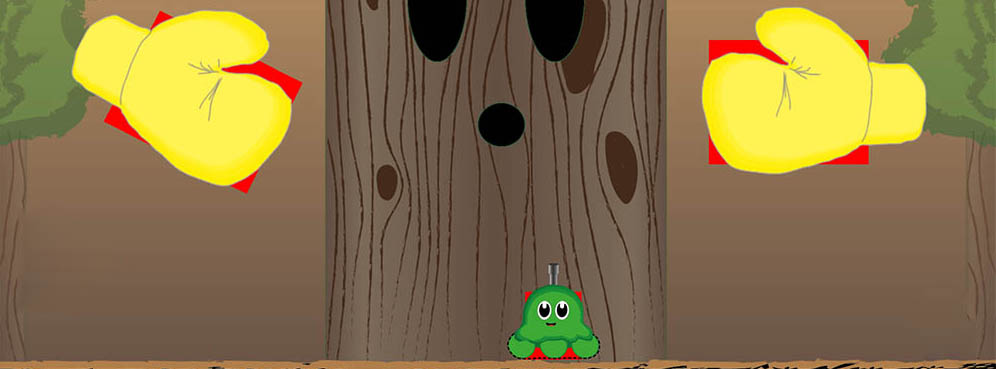
\includegraphics[width=\textwidth - 50pt]{resources/CollisionLayer_BossKampf.jpg}
  \caption{CollisionLayer Debug im Boss Kampf}
  \label{fig:collision_debug_boss} 
\end{figure}

Wenn man genau hinsieht erkennt man, dass auch Münzen über eine Kollision verfügen. Tödliche Objekte in der Karte (bsp. Dornen) jedoch nicht.

\begin{figure}[h]
  \centering
  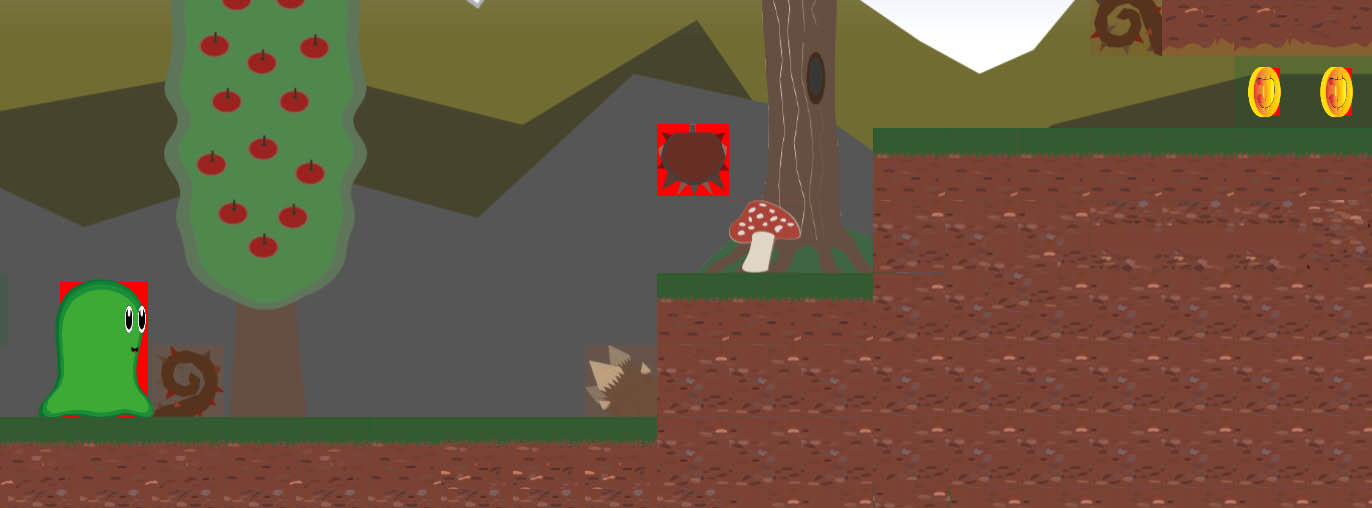
\includegraphics[width=\textwidth - 50pt]{resources/CollisionLayer_Level}
  \caption{CollisionLayer Debug im Level}
  \label{fig:collision_debug_level} 
\end{figure}


\subsection{Listener registrieren}

Die Klasse verfügt über eine Funktion \textbf{setCollisionListener(CollisionLayer*)} die ein anderes Collision Layer als Parameter erwartet. Dabei wird das übergebene Objekt in einer internen Variable gespeichert und in der \textbf{update()} Methode kontinuierlich auf Kollision überprüft.

\subsection{Gegenseite Collision Notification}

Sobald eine Kollision festgestellt wird, werden beide Objekte darüber informiert. Die Methode \textbf{hitByCollision(CollisionLayer*)} ist in der \josieclass{CollisionLayer} Klasse nicht implementiert und muss von den einzelnen Subklassen durch Logik ergänzt werden.

So wird bei einem \josieclass{StageHazard} - im Falle einer Collision mit dem Spieler - das tödliche Objekt wieder auf Anfang positioniert.

\begin{lstlisting}[label=lst:hit_by_collision,
				   language=C++,
				   firstnumber=32,
				   caption=Collision Notification ( StageHazard.cpp )]
void StageHazard::hitByCollision(CollisionLayer* other)
{
	if (other->collisionType == CollisionLayerTypeLevelPlayer) {
		this->fallDown();
	}
}
\end{lstlisting}
(\sectionauthor{OG})
\chapter[Evaluierung]{Evaluierung \small Daniel Mügge}\label{ch:eval}

Im Großen und Ganzen betrachtet ist \gamename ,umgangssprachlich ausgedrückt, ein rundes Ding.
Es gibt einige Dinge die sehr gut glaufen sind, einige Punkte auf die wir nicht unser Hauptaugenmerk gelegt haben und einige die wir einfach vergessen haben. Das kann vielleicht daran liegen das uns viele nützliche Features erst zu Ende des Projektes aufgefallen sind und uns schlicht und ergreifend die Zeit davon gelaufen ist. Zudem wurde JIRA eher schlecht als recht zum managen der Vorgänge und Sprints eingesetzt, wohingegen Git ein nützliches und kontinuierlich verwendetes Tool war.

Die Portierung des Spiels auf andere Plattformen außer Android, wie iOS und OS X, hat bis auf einige kleine Hürden problemlos funktioniert. Speziell für die plattformübergreifende Entwicklung ist cocos2d-x äußerst praktisch, weil die Engine den C$++$-Code selbstständig nativ übersetzt.
Das größte Problem war die unterschiedliche, erlaubte Pixelbreite von Bildern, was aber relativ schnell behoben war.

Auf die integrierte Physiks Engine von cocos2d-x haben wir verzichtet da unser Spiel nur von der Kollision zum Boden Gebrauch macht. Eine normale Physik Engine bezieht dafür noch viel mehr Parameter (bsp. Masse, Momentum, Gravitation) mit ein, was bei uns nicht gegeben ist oder mit einem unnötig hohen Mehraufwand verbunden.

Hinsichtlich der Performance haben wir uns auch wenig Gedanken gemacht. Hier bleibt noch offen Tests anzulegen um bestimmte Kriterien einzuhalten. Oder selbst einfache Tests zwischen zwei Funktionen durchzuführen. Beispielsweise ob es effektiver ist viele kleine Bilder nach Bedarf zu laden oder ein großes Bild ständig im Speicher zu halten. Des weiteren wäre zu klären ob die implementierte Kollisionsabfrage effektiv ist.

Die recht langen Ladezeit beim Starten eines Levels und besonders beim Starten des Zufallslevels sollte mit einem Lade-Bildschirm überdeckt werden, damit für den Endanwender ersichtlich ist, dass etwas im Gange ist.

Als Verbesserung des Ablaufs/Aufbaus der Animationen hätte man die Spawn Klasse von cocos2d-x verwenden können. Dadurch wäre eine variablere Verwendung von Sequenzen und Aktionen möglich. Diese hätte besonders bei den Angriffspattern der Boss Klasse Anwendung gefunden. Dadurch ist die komplette Boss Klasse momentan auf einen einzigen Endgegner fixiert.

Im Hinblick auf die Schwierigkeit und die Balance des Spiels war es für uns als Entwickler besonders schwer das Spiel neutral zu betrachten. Wir haben alles selbst getestet und nach einer gewissen Zeit weiß man eben wie die Levels aussehen und wie die Steuerung einzusetzten ist. An dieser Stelle hätte man gezielte Langzeittests mit Unbeteiligten (sozusagen den Endanwendern) durchführen sollen. Wenn wir es Außenstehenden vorgestellt haben, dann nur kurz nebenbei um zu zeigen wie es aussieht.
Jedoch war bei den kurzen Tests schon zu sehen, dass unser Produkt ein relativ hohes, nennen wir es an dieser Stelle, "'Suchtpotential" hat. Alle Tester \textbf{wollten} die Levels schaffen und waren aufgrund von schwierigeren Passagen nicht gleich demotiviert.
\\Im Bezug auf den Schwierigkeitsgrad ist der Vorteil der "'festen"' Levels gegenüber dem zufällig generiertem Level, dass man diese einfach über den Editor, an Stellen die zu schwer sind, entschärfen kann. Jedoch muss man erwähnen das die Umsetzung des Zufallslevels sehr gut gelungen ist und außerdem wird man natürlich je nach Schwierigkeitsgrad auch mit einer entsprechenden Anzahl an Münzen belohnt(1: 10, 2: 20, 3: 80).

\begin{figure}[H]
\centering
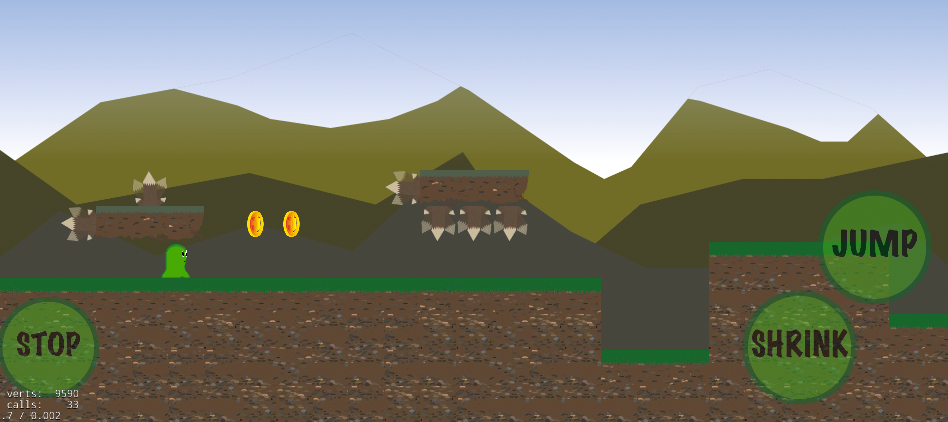
\includegraphics[width=14cm]{resources/randomdiff1}
\\[0.5em]
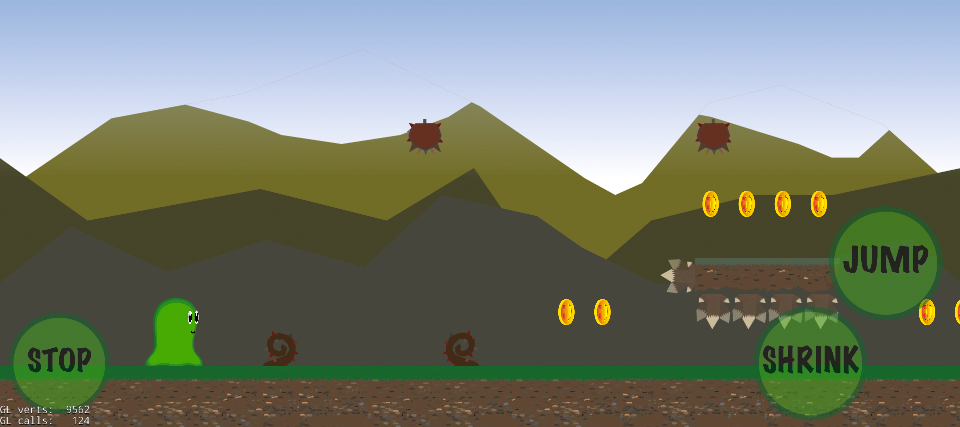
\includegraphics[width=14cm]{resources/randomdiff3}
\caption{Beispiel einer schwierigen Passage zwischen Schwierigkeitsgrad 1 und 3}
\label{fig: randomdiff}
\end{figure}

Die Implementierung des Sprungs bei \gamename ist für Erstanwender möglicherweise etwas gewöhnungsbedürftig, da es keine Mindestsprunghöhe gibt. Es wäre möglich diese zu implementieren jedoch haben wir während der Entwicklung festgestellt, dass das Spiel dadurch eine gewisse Individualität gegenüber anderen Spielen auf dem Markt erhält. Die restlichen Funktionalitäten der Steuerung weisen keine großen Besonderheiten auf und sind selbsterklärend, was sich weder positiv noch negativ auswirkt.

Ein Highlight des Spiels sind die Grafiken. Auch wenn es sich nicht hochkarätige 3D-Grafiken, sondern einfache 2D-Grafiken handelt, harmonieren sie mit dem Gesamtkonzept des Spiels. Sie wurden mit sehr viel Liebe zum Detail gestaltet und strahlen einen gewissen "'niedlichen"' Charme aus. Diese Niedlichkeit ist genau das was wir bei \gamename haben wollten.
Ein gutes Beispiel dafür ist der Shop, in den man gelangt wenn man das Bosslevel startet. 

\begin{figure}[H]
\centering
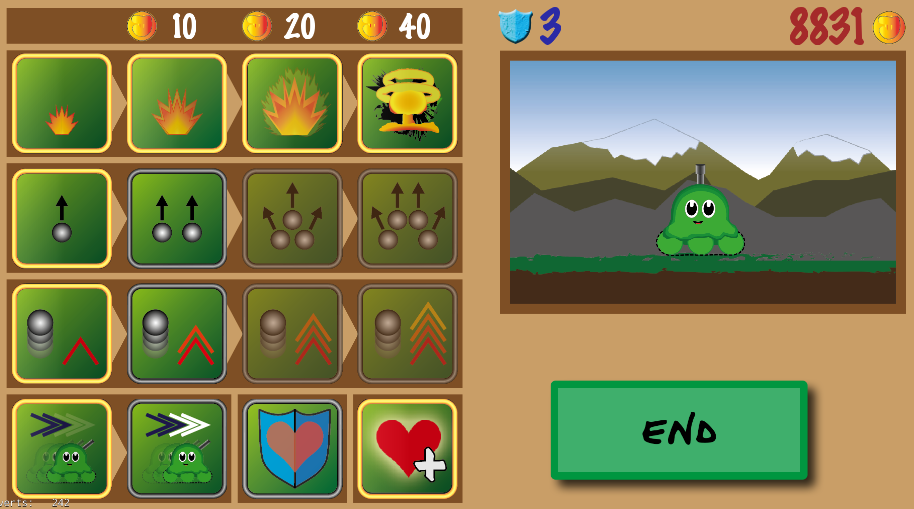
\includegraphics[width=14cm]{resources/shop}
\caption{Shop zum Erwerb von Aufwertungen für das Bosslevel}
\label{fig: shop}
\end{figure}

\chapter{Fazit und Ausblick}

\section{Features for the Future}\label{sec:6_Features}

Aus zeitlichen Gründen konnten wir einige Features nicht umsetzen, dazu gehören:

\begin{itemize}

\item Mehr Levels

Die momentane Levelstruktur 1.1--1.2--1.3--Boss könnte in die vertikale Ebene erweitert werden. In Zukunft wären mehrere Levelebenen wünschenswert. Bedeutet: 2.1--2.2--2.3--Boss 2,  3.1--3.2--3.3--Boss 3 \dots. Durch eine höhere Anzahl von Levels ist auch eine interessante Story mit Cutscenes und neuen Umgebungen besser umsetzbar. 

\item Neue Kampfmodi mit neuen Bossen

Damit ist gemeint, dass Josie sich in einen Hubschrauber verwandeln und den Boss von oben bekämpfen kann oder in einen Mech/Roboter, der anstatt einer Links-Rechts-Bewegung lediglich einen Sprung ausführt und den Boss von der Seite bekämpft.

Neue Bosse mit neuen Angriffspatterns und Bewegungsabläufen, neuen Designs und interessanteren Mechaniken wären eine weitere große Ergänzung die das Spiel noch besser machen würde.

\item Double-Jump-Gliding

Die Erweiterung der Sprungfunktion könnte nach einem weiteren Klick in der Luft dazu führen, dass Josie ein kleines Stück in der Luft gleitet. Das hätte zur Folge dass man auch Levelabschnitte mit größeren Sprungabständen einbauen könnte.

\item Neue Aufwertungsmöglichkeiten

Die bestehenden Aufwertungen im Shop könnte man beispielsweise mit Element--Projektilen, die über verschiedene Schadensarten verfügen und in Abhängigkeit zum Element des Boss Gegners mehr oder weniger Schaden verursachen, erweitern. Hierfür wären auch neue Projektil- -Grafiken erforderlich was das Spiel fürs Auge interessanter machen würde.

\end{itemize}

\chapter{Anhang A}\label{ch:AnhangA}

\begin{figure}[H]
  \centering
  \includegraphics[width=\textwidth]{resources/josieclassdiagramm}
  %\caption{Klassendiagramm}
  %\label{fig:Klassendiagramm} 
\end{figure}


\backmatter
%%%%%%%%%%%%%%%%%%%
%% create figure list
%%%%%%%%%%%%%%%%%%%

\listoffigures
\addcontentsline{toc}{chapter}{Verzeichnisse}			

%%%%%%%%%%%%%%%%%%%
%% create tables list
%%%%%%%%%%%%%%%%%%%
\listoftables

%%%%%%%%%%%%%%%%%%%
%% create listings list
%%%%%%%%%%%%%%%%%%%
\lstlistoflistings
\addcontentsline{toc}{chapter}{Listings}				

\printbibliography
\addcontentsline{toc}{chapter}{Literatur}				
\end{document}


